\documentclass[a4paper]{article}

\usepackage{cmap}
\usepackage{tabularx}
\usepackage[pdftex]{graphicx}
\graphicspath{{pic/}}

\usepackage[T2A]{fontenc}
\usepackage[utf8]{inputenc}
\usepackage[english,russian]{babel}
\usepackage{amsmath,amssymb}
\usepackage{listings}
\usepackage{color}

\usepackage[top = 20mm, left = 30mm, bottom = 20mm, right = 15mm]{geometry}

\begin{document}
\begin{titlepage}
\begin{center}
\begin{center}
  
\includegraphics[width = 2cm]{logo_mirea.png}
\end{center}
\Large МИНОБРНАУКИ РОССИИ \\
\Large Федеральное государственное бюджетное образовательное учреждение\\
\Large высшего профессионального образования\\
\Large "Московский государственный технический университет радиотехники,\\
\Large электроники и автоматики"\\
\LARGE \bf МТУ МИРЭА \\
\end{center}

\vspace{8em}

\begin{center}
\Large
Методическое пособие\\
по выполнению лабораторных работ по дисциплине\\
«Программные средства ЭВМ»\\
Власов Е.Е.\\
\end{center}

\end{titlepage}

\large
\tableofcontents
\Large
\newpage
\section{\bf Аннотация.}
Выполнение обучающимися лабораторных работ проводится с целью:
\begin{itemize}
  \item формирования практических умений в соответствии с требованиями к уровню подготовки обучающихся, 
  установленными рабочей программой дисциплины/профессионального модуля по конкретным \\
  разделам/темам дисциплин или междисциплинарных курсов;
  \item обобщения, систематизации, углубления, закрепления полученных теоретических знаний;
  \item совершенствования умений применять полученные знания на практике, реализации единства интеллектуальной и практической деятельности;  
  \item развития интеллектуальных умений у будущих специалистов: аналитических, проектировочных, конструктивных и др.;
  \item выработки таких профессионально значимых качеств, как самостоятельность, ответственность, точность, творческая инициатива при
решении поставленных задач при освоении общих компетенций.
\end{itemize}
\newpage
\section{\bf Лабораторная работа №1. Процессы}
\subsection{\Large Понятие процесса.}
\rm Рассмотрим следующий пример. Два студента запускают программу извлечения квадратного корня. Один хочет вычислить квадратный корень из 4, а второй – из 1. С точки зрения студентов, запущена одна и та же программа; с точки зрения компьютерной системы,запущено два различных вычислительных процесса, так как разные исходные данные приводят к разному набору вычислений. Следовательно, на уровне происходящего внутри вычислительной системы, нельзя использовать термин "программа" в пользовательском смысле слова. \\\\
Для выполнения программы, ОС должна выделить определенное количество оперативной памяти, закрепить за ней определенные устройства ввода-вывода или файлы (откуда должны поступать входные данные и куда нужно доставить полученные результаты), то есть зарезервировать определенные ресурсы из общего числа ресурсов всей вычислительной системы. Их количество и конфигурация с течением времени могут изменяться. Для описания таких активных объектов внутри компьютерной системы вместо терминов "программа" и "задание" используют термин – "процесс".\\\\
Понятие процесса характеризует некоторую совокупность набора исполняющихся команд, ассоциированных с ним ресурсов (выделенная для исполнения память или адресное пространство, стеки, используемые файлы и устройства ввода-вывода и т. д.) и текущего момента его выполнения (значения регистров, программного счетчика, состояние стека и значения переменных), находящуюся под управлением операционной системы. Не существует взаимно-однозначного соответствия между процессами и программами, обрабатываемыми вычислительными системами. Как будет показано далее, в некоторых операционных системах для работы определенных программ может организовываться более одного процесса или один и тот же процесс может исполнять последовательно несколько различных программ. Более того, даже в случае обработки только одной программы в рамках одного процесса нельзя считать, что процесс представляет собой просто динамическое описание кода исполняемого файла, данных и выделенных для них ресурсов. Процесс находится под управлением операционной системы, поэтому в нем может выполняться часть кода ее ядра (не находящегося в исполняемом файле!), как в случаях, специально запланированных авторами программы (например, при использовании системных вызовов), так и в непредусмотренных ситуациях (например, при обработке внешних прерываний).

\subsection{\Large Состояние процесса.}
\rm В операционных системах, которые поддерживают концепцию процессов, всё, что выполняется в вычислительной системе (не только программы пользователей, но и, возможно, определенные части операционной системы), организовано как набор процессов. Понятно, что реально на однопроцессорной компьютерной системе в каждый момент времени может исполняться только один процесс. Для мультипрограммных вычислительных систем псевдопараллельная обработка нескольких процессов достигается с помощью переключения процессора с одного процесса на другой. Пока один процесс выполняется, остальные ждут своей очереди выполнения.\\\\
Очевидно, что процесс может находится как минимум в двух состояниях «Выполнение» и «Ожидание».\\\\
Процесс, который находится в состоянии «Выполнение», через некоторое время может быть завершен операционной системой или приостановлен и снова переведен в состояние «Ожидание». Приостановка процесса происходит по двум причинам: для его дальнейшей работы потребовалось какое-либо событие (например, завершение операции ввода-вывода) или истек квант времени, отведенный операционной системой для работы данного процесса. После перевода процесса в состояние «Ожидание» ОС по определенному алгоритму выбирает для исполнения один из процессов, находящихся в состоянии «Ожидание», и переводит его в состояние «Выполнение». Новый процесс, созданный в системе, первоначально помещается в состояние «Ожидание».\\\\
Это очень грубая модель, она не учитывает, в частности, то, что процесс, выбранный для исполнения, может все еще ждать события, из-за которого он был приостановлен, и реально к выполнению не готов. Для того чтобы избежатьтакой ситуации, разобьем состояние «Ожидание» на два новых состояния: «Готов к запуску» и «Сон».\\\\
После этого уточнения каждый новый процесс, созданный в системе, попадает в состояние «Готов к запуску». ОС, пользуясь каким-либо алгоритмом планирования, выбирает один из готовых процессов и переводит его в состояние «Выполнение». В состоянии «Выполнение» происходит непосредственное выполнение программного кода процесса. Выполнение процесса может происходить в двух режимах: в режиме ядра и в режиме задачи.\\\\
Выйти из этого состояния процесс может по трем причинам: 
\begin{enumerate}
  \item программа, выполняемая в процессе, закончила исполнение и/или ОС прекращает работу процесса;
  \item он не может продолжать свою работу, пока не произойдет некоторое событие, и ОС переводит его в состояние «Сон»;
  \item в результате возникновения прерывания в вычислительной системе (например, прерывания от таймера по истечении предусмотренного времени выполнения) его возвращают в состояние «Готов к запуску».
\end{enumerate}
Из состояния «Сон» процесс попадает в состояние «Готов к запуску» после того, как ожидаемое событие произошло, и он снова может быть выбран для исполнения. \\\\
Такая модель хорошо описывает поведение процессов во время их существования, но она не уделяет внимание созданию процесса в системе и его удалению. Для полноты картины нам необходимо ввести еще два состояния процессов: «Создан» и «Зомби». \\\\
Теперь, для появления в вычислительной системе, процесс должен пройти через состояние «Создан». При создании процесс получает в свое распоряжение адресное пространство, в которое загружается код программы; ему выделяются стек и системные ресурсы; устанавливается начальное значение программного счетчика этого процесса и т. д. Созданный процесс переводится в состояние «Готов к запуск». При завершении своей работы процесс из состояния исполнение попадает в состояние «Зомби».

\subsection{\Large Операции над процессами и связанные с ними понятия.}
Процесс не может перейти из одного состояния в другое самостоятельно. Изменением состояния процессов занимается ОС, совершая операции над ними. Количество таких операций в нашей модели пока совпадает с количеством стрелок на диаграмме состояний. Удобно объединить их в три пары:
\begin{enumerate}
  \item создание процесса – завершение процесса;
  \item приостановка процесса (перевод из состояния исполнение в состояние готовность) – запуск процесса (перевод из состояния готовность в состояние исполнение);
  \item блокирование процесса (перевод из состояния исполнение в состояние ожидание) – разблокирование процесса (перевод из состояния ожидание в состояние готовность).
\end{enumerate}
Также существует еще одна операция, не имеющая парной: изменение приоритета процесса. \\\\
Операции создания и завершения процесса являются однократными, так как могут быть применены к процессу не более одного раза (некоторые системные процессы при работе вычислительной системы не завершаются никогда). Все остальные операции, связанные с изменением состояния процессов, будь то запуск или блокировка, как правило, являются многократными.

\subsubsection{\Large Process Control Block и контекст процесса.}
Для того чтобы ОС могла выполнять операции над процессами, каждый процесс представляется в ней некоторой структурой данных. Эта структура содержит информацию, специфическую для данного процесса:
\begin{itemize}
  \item состояние, в котором находится процесс;
  \item программный счетчик процесса (адрес команды, которая должна быть выполнена для него следующей);
  \item содержимое регистров процессора;
  \item данные, необходимые для планирования использования процессора и управления памятью (приоритет процесса, размер и расположение адресного пространства и т. д.);
  \item учетные данные (идентификационный номер процесса, какой пользователь инициировал его работу, общее время использования процессора данным процессом и т.д.);
  \item сведения об устройствах ввода-вывода, связанных с процессом (например, какие устройства закреплены запроцессом, таблицу открытых файлов).
\end{itemize}
Состав и строение этой структуры зависят от конкретной операционной системы. Во многих операционных системах информация, характеризующая процесс, хранится не в одной, а в нескольких связанных структурах данных. Эти структуры могут иметь различные наименования, содержать дополнительную информацию или, наоборот, лишь часть описанной информации. В принципе, это не играет особой роли для понимания работы операционной системы с процессами. Главное то, что для любого процесса, находящегося в ОС, вся информация, необходимая для совершения операций над ним хранится в виде некой (возможно не одной) структуры данных. Мы будем называть ее \bf PCB \rm(Process Control Block) или блоком управления процессом. Блок управления процессом является моделью процесса для операционной системы. Любая операция, производимая операционной системой над процессом, вызывает определенные изменения в \bf PCB.\\\\
PCB \rm можно разделить на две части:
\begin{enumerate}
  \item контекст процесса;
  \item контекст ядра;
\end{enumerate}
Под пользовательским контекстом процесса понимают код и данные, расположенные в адресном пространстве процесса. Все данные подразделяются на:
\begin{itemize}
  \item инициализируемые неизменяемые данные (например, константы);
  \item инициализируемые изменяемые данные (все переменные, начальные значения которых присваиваются на этапе компиляции);
  \item неинициализируемые изменяемые данные (все статические переменные, которым не присвоены начальные значения на этапе компиляции);
  \item стек пользователя;
  \item  данные, расположенные в динамически выделяемой памяти (например, с помощью стандартных библиотечных C функций malloc(), calloc(), realloc()).
\end{itemize}
Контекст ядра содержит информацию, которая необходима ОС для управления процессом.\\
В любой момент времени процесс полностью характеризуется своим контекстом.\\
Сложный жизненный путь процесса в компьютере начинается с его рождения. Любая ОС, поддерживающая концепцию процессов, должна обладать средствами для их создания. В очень простых системах (например, в системах, спроектированных для работы только одного конкретного приложения) все процессы могут быть порождены на этапе старта системы. Более сложные операционные системы создают процессы динамически, по мере необходимости. Инициатором создания нового процесса после старта операционной системы может выступить либо процесс пользователя, совершивший специальный системный вызов, либо сама ОС, то есть, в конечном итоге, тоже некоторый процесс. Процесс, инициировавший создание нового процесса, принято называть родительским процессом (parent process), а вновь созданный процесс – дочерним процессом (child process). Дочерние процессы могут в свою очередь создавать новых детей и т. д., образуя, в общем случае, внутри системы набор генеалогических деревьев процессов – генеалогический лес. Следует отметить, что все пользовательские процессы вместе с некоторыми процессами операционной системы принадлежат одному и тому же дереву леса. В ряде вычислительных систем лес вообще вырождается в одно такое дерево.\\\\
При создания процесса система заводит новый \bf PCB \rm с состоянием процесса «Создан» и начинает его заполнять. Новый процесс получает собственный уникальный идентификационный номер – Process Identificator - PID. В ОС Unix для хранения PID используется переменная типа pid\_t, размерность которой совпадает с разрядностью самой системы. PID нового процесса больше PID последнего созданного процесса или, в случае если PID превышает максимальный, первому свободному. После завершения какого-либо процесса его освободившийся PID может быть повторно использован для другого процесса. Обычно для выполнения своих функций дочерний процесс требует определенных ресурсов: памяти, файлов, устройств ввода-вывода и т. д. Существует два подхода к их выделению. Новый процесс может получить в свое распоряжение некоторую часть родительских ресурсов, возможно разделяя с процессом-родителем и другими процессами-детьми права на них, или может получить свои ресурсы непосредственно от операционной системы. Информация о выделенных ресурсах заносится в \bf PCB.\\\\
\rm После того, как система выделила необходимые ресурсыновому процессу, происходит загрузка вадресное пространство процесса код программы и данных. Устанавливается программный счетчик. Здесь также возможны два решения. В первом случае дочерний процесс становится дубликатом процесса-родителя \bf PCB \rm(за исключением PID и некоторых других данных (подробнее см.). Во втором случае дочерний процесс загружается новой программой из какого-либо файла. ОС Unix разрешает порождение процесса только первым способом: для запуска новой программы необходимо сначала создать копию родительского процесса, а затем дочерний процесс должен заменить свой пользовательский контекст с помощью специального системного вызова. Создание нового процесса как дубликата процесса- родителя приводит к возможности существования программ (т.е. исполняемых файлов), для работы которых организуется более одного процесса.
Возможность замены пользовательского контекста процесса по ходу его работы (т.е. загрузки для исполнения новой программы) приводит к
тому, что на протяжении жизни одного и того же процесса в нем может последовательно выполняться несколько различных программ.\\\\
После того как процесс наделен содержанием, в \bf PCB \rm дописывается оставшаяся информация, и ОС переводит процесс в состояние «Готов к запуску». Осталось сказать несколько слов о том, как ведут себя родительские процессы после создании дочерних процессов. Родительский процесс может продолжать свое выполнение одновременно с выполнением дочернего процесса, а может ожидать завершения работы некоторых или всех своих "детей". \\
После того как процесс завершил свою работу, ОС переводит его в состояние «Зомби» и освобождает все ассоциированные с ним ресурсы, делая соответствующие записи в блоке управления процессом. При этом сам PCB не уничтожается, а остается в системе еще некоторое время. Это связано с тем, что родительский процесс после завершения дочернего процесса может запросить ОС о причине "смерти" порожденного им процесса и/или статистическую информацию
о его работе. Подобная информация сохраняется в PCB отработавшего процесса до запроса процесса-родителя или до
конца его деятельности, после чего все следы завершившегося процесса окончательно исчезают из системы.\\
Дочерний процесс могут продолжать работу после того, как их родительский процесса завершил свое выполнение. В этом случае дочерний процесс "усыновляются" одним из системных процессов, который порождается при старте операционной системы и функционирует все время, пока она работает.

\subsection{\Large Многократные операции.}
Однократные операции приводят к изменению количества процессов, находящихся под управлением операционной системы, и всегда связаны с выделением или освобождением определенных ресурсов. Многократные операции, напротив, не приводят к изменению количества процессов в ОС и не обязаны быть связанными с выделением или освобождением ресурсов.\\\\
\bf Запуск процесса. \rm Из числа процессов, находящихся в состоянии готовность, ОС выбирает один процесс для последующего исполнения. Критерии и алгоритмы такого выбора будут подробно рассмотрены в лекции 3 – "Планирование процессов". Для избранного процесса ОС обеспечивает наличие в оперативной памяти информации, необходимой для его дальнейшего выполнения. То, как она это делает, будет в деталях описано в лекциях 8-10. Далее состояние процесса изменяется на исполнение, восстанавливаются значения регистров для данного процесса и управление передается команде, на которую указывает счетчик команд процесса. Все данные, необходимые для восстановления контекста, извлекаются из PCB процесса, над которым совершается операция.\\\\
\bf Приостановка процесса. \rm Работа процесса, находящегося в состоянии исполнение, приостанавливается в результате
какого-либо прерывания. Процессор автоматически сохраняет счетчик команд и, возможно, один или несколько регистров в стеке исполняемого процесса, а затем передает управление по специальному адресу обработки данного прерывания. На этом деятельность hardware по обработке прерывания завершается. По указанному адресу обычно располагается одна из частей операционной системы. Она сохраняет динамическую часть системного и регистрового контекстов процесса в его PCB, переводит процесс в состояние «готовность» и приступает к обработке прерывания, то есть к выполнению определенных действий, связанных с возникшим прерыванием.\\\\
\bf Блокировка процесса. \rm Процесс блокируется, когда он не может продолжать работу, не дождавшись возникновения какого-либо события в вычислительной системе. Для этого он обращается к ОС с помощью определенного системного вызова. ОС обрабатывает системный вызов (инициализирует операцию ввода-вывода, добавляет процесс в очередь процессов, дожидающихся освобождения устройства или возникновения события, и т. д.) и, при необходимости сохранив нужную часть контекста процесса в его PCB, переводит процесс из состояния исполнение в состояние ожидание.\\\\
\bf Разблокировка процесса. \rm После возникновения в системе какого-либо события ОС нужно точно определить, какое именно событие произошло. Затем ОС проверяет, находился ли некоторый процесс в состоянии ожидание для данного события, и если находился, переводит его в состояние готовность, выполняя необходимые действия, связанные с наступлением события (инициализация операции ввода-вывода для очередного ожидающего процесса и т. п.).

\subsection{\Large Переключение контекста.}
До сих пор мы рассматривали операции над процессами изолированно, независимо друг от друга. В действительности же деятельность мультипрограммной операционной системы состоит из цепочек операций, выполняемых над различными процессами, и сопровождается переключением процессора с одного процесса на другой.\\\\
Давайте, для примера, упрощенно рассмотрим, как в реальности может протекать операция разблокирования процесса, ожидающего ввода-вывода.
\begin{center}
  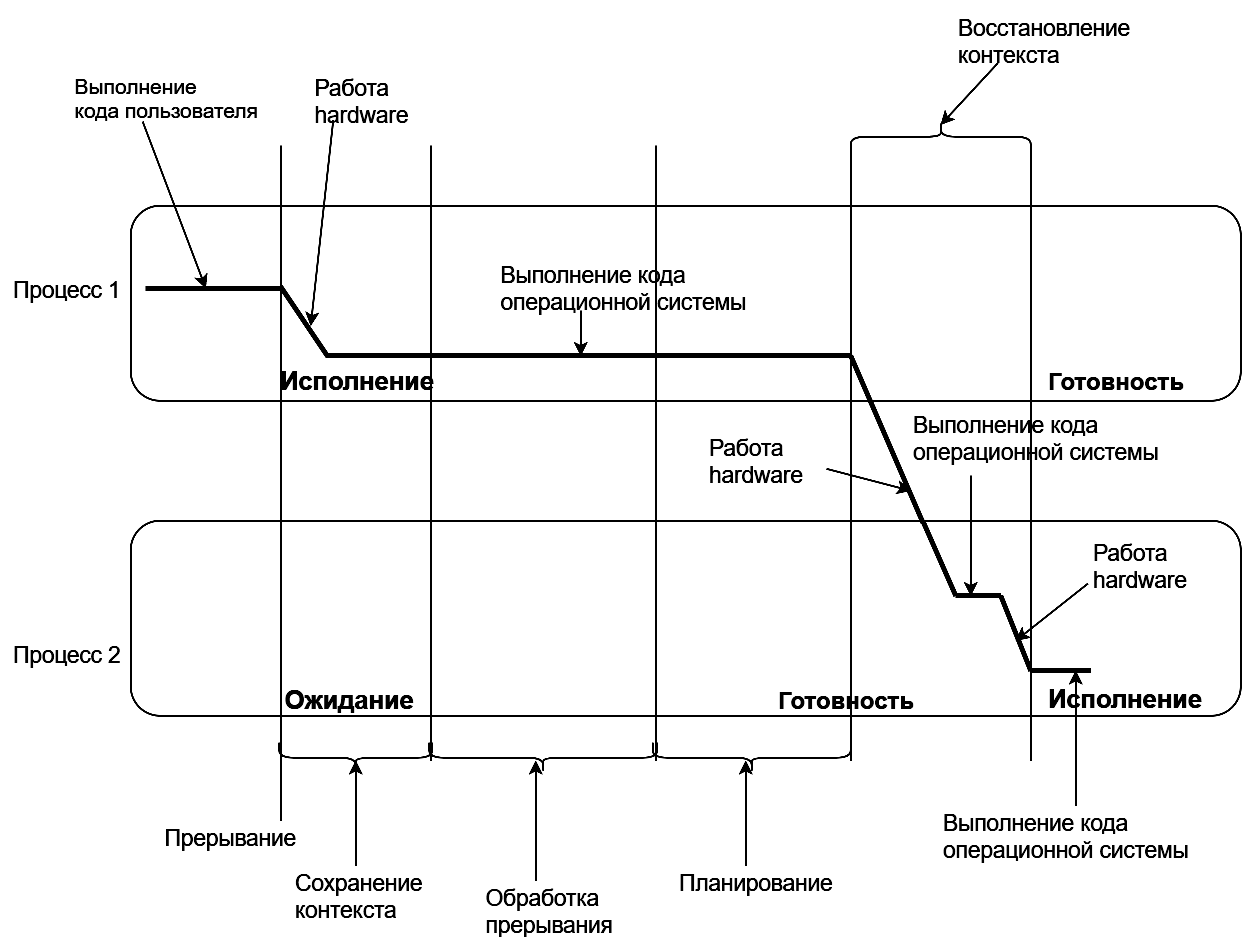
\includegraphics[width = 16cm]{os.png}
\end{center}
При исполнении процессором некоторого процесса (на рисунке – процесс 1) возникает прерывание от устройства ввода- вывода, сигнализирующее об окончании операций на устройстве. Над выполняющимся процессом производится операция приостановки. Далее ОС разблокирует процесс, инициировавший запрос на ввод-вывод (на рисунке – процесс 2) и осуществляет запуск приостановленного или нового процесса, выбранного при выполнении планирования (на рисунке был выбран разблокированный процесс). Как мы видим, в результате обработки информации об окончании операции ввода-вывода возможна смена процесса,находящегося в состоянии исполнение.\\\\
Для корректного переключения процессора с одного процесса на другой необходимо сохранить контекст исполнявшегося процесса и восстановить контекст процесса, на который будет переключен процессор. Такая процедура сохранения/восстановления работоспособности процессов называется переключением контекста. Время, затраченное на переключение контекста, не используется вычислительной системой для совершения полезной работы и представляет собой накладные расходы, снижающие производительность системы. Оно меняется от машины к машине и обычно колеблется в диапазоне от 1 до 1000 микросекунд. Существенно сократить накладные расходы в современных операционных системах позволяет расширенная модель процессов, включающая в себя понятие threads of execution (нити исполнения или просто нити).

\subsection{\Large Системные вызовы работы с процессами}
\subsubsection{\Large Получение информации о процессе. Системные вызовы getppid() и getpid().}
Данные ядра, находящиеся в контексте ядра процесса, не могут быть прочитаны процессом непосредственно. Для получения информации о них процесс должен совершить соответствующий системный вызов. Значение идентификатора текущего процесса может быть получено с помощью системного вызова getpid(), а значение идентификатора родительского процесса для текущего процесса – с помощью системного вызова getppid(). Прототипы этих системных вызовов и соответствующие типы данных описаны в системных файлах <sys/types.h> и <unistd.h>. Системные вызовы не имеют параметров и возвращают идентификатор текущего процесса и идентификатор родительского процесса
соответственно. \\\\
\sl Прототипы системных вызовов:
\begin{verbatim}
#include <sys/types.h>
#include <unistd.h>
pid_t getpid(void);
pid_t getppid(void);
\end{verbatim}
\sl Описание системных вызовов:\\
\rm Системный вызов getpid возвращает идентификатор текущего процесса. Системный вызов getppid возвращает идентификатор процесса-родителя для текущего процесса. Тип данных pid\_t является синонимом для одного из целочисленных типов языка C. Написание программы с использованием getpid() и getppid().\\\\
В качестве примера использования системных вызовов getpid() и getppid() самостоятельно напишите программу, печатающую значения PID и PPID для текущего процесса. Запустите ее несколько раз подряд. Посмотрите, как меняется идентификатор текущего процесса. Объясните наблюдаемые изменения.

\subsubsection{\Large Создание процесса в UNIX. Системный вызов fork().}
В ОС UNIX новый процесс может быть порожден единственным способом – с помощью системного вызова fork(). При этом вновь созданный процесс будет являться практически полной копией родительского процесса. У порожденного процесса по сравнению с родительским
процессом (на уровне уже полученных знаний) изменяются значения следующих параметров:
\begin{itemize}
  \item идентификатор процесса – PID;
  \item идентификатор родительского процесса – PPID.
\end{itemize}
Дополнительно может измениться поведение порожденного процесса по отношению к некоторым сигналам.\\\\
\bf Системный вызов fork(). \\
\sl Прототип системного вызова:
\begin{verbatim}
#include <sys/types.h>
#include <unistd.h>
pid_t fork()(void);
\end{verbatim}
\sl Описание системного вызова:
\rm Системный вызов fork() служит для создания нового процесса в ОС UNIX. Процесс, который инициировал системный вызов fork(), принято называть родительским процессом (parent process). Вновь порожденный процесс принято называть процессом-ребенком (child process). Дочерний процесс является почти полной копией родительского процесса. У порожденного процесса по сравнению с родительским изменяются значения следующих параметров:
\begin{itemize}
  \item идентификатор процесса;
  \item идентификатор родительского процесса;
  \item время, оставшееся до получения сигнала SIGALRM;
  \item сигналы, ожидавшие доставки родительскому процессу, не будут доставляться порожденному процессу.
\end{itemize}
При однократном системном вызове возврат из него может произойти дважды: один раз в родительском процессе, а второй раз в порожденном процессе. Для того чтобы после возвращения из системного вызова fork() процессы могли определить, какой из них является дочерним, а какой родительским, и, соответственно, по-разному организовать свое поведение, fork() возвращает в них разные значения. Если создать новый процесс не удалось, то системный вызов вернет в инициировавший его процесс отрицательное значение.\\\\
Системный вызов fork() является единственным способом породить новый процесс после инициализации операционной системы UNIX.

\subsubsection{\Large Завершение процесса. Функция exit().}
Существует два способа корректного завершения процесса в программах, написанных на языке C. Первый способ мы использовали до сих пор: процесс корректно завершался по достижении конца функции main() или при выполнении оператора return в функции main(), второй способ применяется при необходимости завершить процесс в каком-либо другом месте программы. Для этого используется функция exit() из стандартной библиотеки функций для языка C. При выполнении этой функции происходит сброс всех частично заполненных буферов ввода-вывода с закрытием соответствующих потоков, после чего инициируется системный вызов прекращения работы процесса
и перевода его в состояние \bf закончил исполнение.
\rm Возврата из функции в текущий процесс не происходит и функция ничего не возвращает. Значение параметра функции exit() – кода завершения процесса – передается ядру операционной системы и может быть затем получено процессом, породившим завершившийся процесс. На самом деле при достижении конца функции main() также неявно вызывается эта функция со значением параметра 0.
Функция для нормального завершения процесса:\\
Прототип функции:
\begin{verbatim}
#include <stdlib.h>
void exit()(int status);
\end{verbatim}
\sl Описание функции:\\
\rm Функция exit() служит для нормального завершения процесса. При выполнении этой функции происходит сброс всех частично заполненных буферов ввода-вывода с закрытием соответствующих потоков (файлов, pipe, FIFO, сокетов), после чего инициируется системный вызов прекращения работы процесса и перевода его в состояние закончил исполнение. \\\\
Возврата из функции в текущий процесс не происходит, и функция ничего не возвращает. \\\\
Значение параметра status – кода завершения процесса – передается ядру операционной системы и может быть затем получено процессом, породившим завершившийся процесс. При этом используются только младшие 8 бит параметра, так что для кода завершения допустимы значения от 0 до 255. По соглашению, код завершения 0 означает безошибочное завершение процесса.\\\\
Для изменения пользовательского контекста процесса применяется системный вызов exec(), который пользователь не может вызвать непосредственно. Вызов exec() заменяет пользовательский контекст текущего процесса на содержимое некоторого исполняемого файла и устанавливает начальные значения регистров процессора (в том числе устанавливает программный счетчик на начало загружаемой программы). Этот вызов требует для своей работы задания имени исполняемого файла, аргументов командной строки и параметров окружающей среды. Для осуществления вызова программист может воспользоваться одной из шести функций: execlp(), execvp(), execl() и, execv(), execle(), execve() отличающихся друг от друга представлением параметров, необходимых для работы системного вызова exec().\\\\
Функции изменения пользовательского контекста процесса:\\
\sl Прототипы функций:
\begin{verbatim}
#include <unistd.h>
int execlp(const char *file,
           const char *arg0,
           ... const char *argN,(char *)NULL)

int execvp(const char *file, char *argv[])

int execl(const char *path,const char *arg0,
          ... const char *argN,(char *)NULL)

int execv(const char *path, char *argv[])

int execle(const char *path,
           const char *arg0,
           ... const char *argN, (char *)NULL,
           char * envp[])

int execve(const char *path, char *argv[],
           char *envp[])
\end{verbatim}
\sl Описание функций:\\
\rm Для загрузки новой программы в системный контекст текущего процесса используется семейство взаимосвязанных функций, отличающихся друг от друга формой представления параметров. \\
Аргумент file является указателем на имя файла, который должен быть загружен. Аргумент path – это указатель на полный путь к файлу, который должен быть загружен. \\
Аргументы arg0, ..., argN представляют собой указатели на аргументы командной строки. Заметим, что аргумент arg0 должен указывать на имя загружаемого файла. \\
Аргумент argv представляет собой массив из указателей на аргументы командной строки. Начальный элемент массива должен указывать на имя загружаемой программы, а заканчиваться массив должен элементом, содержащим указатель NULL. \\
Аргумент envp является массивом указателей на параметры окружающей среды, заданные в виде строк «переменная=строка». Последний элемент этого массива должен содержать указатель NULL. \\\\
Поскольку вызов функции не изменяет системный контекст текущего процесса, загруженная программа унаследует от загрузившего ее процесса следующие атрибуты:
\begin{itemize}
  \item идентификатор процесса;
  \item идентификатор родительского процесса;
  \item групповой идентификатор процесса;
  \item идентификатор сеанса;
  \item время, оставшееся до возникновения сигнала SIGALRM;
  \item текущую рабочую директорию;
  \item маску создания файлов;
  \item идентификатор пользователя;
  \item групповой идентификатор пользователя;
  \item явное игнорирование сигналов;
  \item таблицу открытых файлов (если для файловогодескриптора не устанавливался признак «закрыть файл при выполнении exec()»).
\end{itemize}
В случае успешного выполнения возврата из функций в программу, осуществившую вызов, не происходит, а управление передается загруженной программе. В случае неудачного выполнения в программу, инициировавшую вызов, возвращается отрицательное значение. \\\\
Поскольку системный контекст процесса при вызове exec() остается практически неизменным, большинство атрибутов процесса, доступных пользователю через системные вызовы (PID, UID, GID, PPID и другие, смысл которых станет понятен по мере углубления наших знаний на дальнейших занятиях), после запуска новой программы также не изменяется.\\\\
\bf Важно понимать разницу между системными вызовами fork() и exec(). Системный вызов fork() создает новый процесс, у которого пользовательский контекст совпадает с пользовательским контекстом процесса-родителя. Системный вызов exec() изменяет пользовательский контекст текущего процесса, не создавая новый процесс.

\subsubsection{\Large Системный вызов wait/waitpid().}
\begin{verbatim}
#include <sys/types.h>
#include <sys/wait.h>
pid_t wait(int *status);
pid_t waitpid(pid_t pid, int *status, int options);
\end{verbatim}
\rm Функция \bf wait \rm приостанавливает выполнение текущего процесса до тех пор, пока дочерний процесс не завершится, или до появления сигнала, который либо завершает текущий процесс, либо требует вызвать функцию- обработчик. Если дочерний процесс к моменту вызова функции уже завершился (так называемый "зомби" ("zombie")), то функция немедленно возвращается. Системные ресурсы, связанные с дочерним процессом, освобождаются. Функция \bf waitpid \rm приостанавливает выполнение текущего процесса до тех пор, пока дочерний процесс, указанный в параметре pid, не завершит выполнение, или пока не появится сигнал, который либо завершает текущий процесс либо требует вызвать функцию-обработчик. Если указанный дочерний процесс к моменту вызова функции уже завершился (так называемый "зомби"), то функция немедленно возвращается. Системные ресурсы, связанные с дочерним процессом, освобождаются. Параметр pid может принимать несколько значений:\\\\
\begin{tabular}{p{2cm}p{13cm}}
\bf < -1 & \rm означает, что нужно ждать любого дочернего процесса, идентификатор группы процессов которого равен абсолютному значению pid.\\
\bf -1 & \rm означает ожидание любого дочернего процесса; функция wait ведет себя точно так же.\\
\bf 0 & \rm означает ожидание любого дочернего процесса, идентификатор группы процессов которого равен идентификатору текущего процесса.\\
\bf > 0 & \rm означает ожидание дочернего процесса, чей идентификатор равен pid.\\
\end{tabular}
\\\\
Значение \sl options \rm создается путем логического сложения нескольких следующих констант:\\
\bf WNOHANG\\
\rm означает немедленное возвращение управления, если ни один дочерний процесс не завершил выполнение.\\\\
\bf WUNTRACED\\
\rm означает возврат управления и для остановленных (но не отслеживаемых) дочерних процессов, о статусе которых еще не было сообщено. Статус для отслеживаемых остановленных подпроцессов также обеспечивается без этой опции.\\\\
ВОЗВРАЩАЕМЫЕ ЗНАЧЕНИЯ:\\
Возвращает идентификатор дочернего процесса, который завершил выполнение, или ноль, если использовался WNOHANG и ни один дочерний процесс пока еще недоступен, или -1 в случае ошибки (в этом случае переменной errno присваивается соответствующее значение).\\\\
\sl НАЙДЕННЫЕ ОШИБКИ:\\
\begin{tabular}{p{2cm}p{13cm}}
  \bf ECHILD & \rm Процесс, указанный в pid, не существует или не является дочерним процессом текущего процесса. (Это может случиться и с собственным дочерним процессом, если обработчик сигнала SIGCHLD установлен в SIG\_IGN. Смотри также главу ЗАМЕЧАНИЯ по поводу многозадачности процессов.) \\\\
  \bf EINVAL & \rm Аргумент \sl options \rm неверен.\\\\
  \bf EINTR & \rm Использовался флаг WNOHANG, и был получен необработанный сигнал или SIGCHLD. Стандарт Single Unix Specification описывает флаг SA\_NOCLDWAIT (не поддерживается в Linux), если он установлен или обработчик сигнала SIGCHLD устанавливается в SIG\_IGN, то завершившиеся дочерние процессы не становятся зомби, а вызов wait()или waitpid() блокируется, пока все дочерние процессы не завершатся.
\end{tabular}
\\\\
\rm
Стандарт POSIX оставляет неопределенным поведение при установке \\SIGCHLD в SIG\_IGN. поздние стандарты, включая SUSv2 и 
\\ POSIX 1003.12001, определяют поведение, только что описанное как опция совместимости с XSI. Linux не следует второму варианту: если вызов wait() или waitpid() сделан в то время, когда SIGCHLD игнорируется, то вызов ведет себя, как если бы SIGCHLD не игнорировался, то есть вызов блокирует до завершения работы следующего подпроцесса и возврата идентификатора процесса PID и статуса этого подпроцесса.

\newpage
\section{Лабораторная работа №2. Файлы}
\subsection{\Large Теоретическое введение.}
Файл - это сущность, позволяющая получить доступ к какому-либо ресурсу вычислительной системы.\\
В большинстве случаев файл определяет именованную область на устройстве хранения данных. В unix-like операционных системах файлом является
большинство ресурсов вычислительной системы. В UNIX и POSIX - системах сущствуют следующие типы файлов:
\begin{itemize}
  \item Обычный файл
  \item Каталог
  \item FIFO-файл
  \item Символическая ссылка
  \item Байт-ориентированный файл устройства
  \item Блок-ориентированный файл устройства.
\end{itemize}
\sl Обычный файл \rm может быть тестовым и двоичным. В unix системах эти типы файлов не различаются и оба могут быть «исполняемыми» при условии, что на них установлено разрешение на выполнение и они могут читаться и записываться пользователем, имеющим соответствующие права доступа.\\\\
\sl FIFO-файл \rm является специальным файлом, который предназначен для организации обмена данными между процессами.\\\\
\sl Символическая ссылка \rm содержит путевое имя, которое обозначает другой файл в файловой системе.\\\\
\sl Каталог \rm содержит файлы и каталоги. Концепция каталога позволяет организовать файлы в некоторую иерархическую структуру. В Unix ситемах базовым является каталог ‘/’.\\\\
\sl Блок-ориентированные файл \rm устройства служит для предствления физического устройства, которое передает данные блоками. Примерами таких устройств являются жесткие диски.\\\\
\sl Байт-ориентированный файл \rm устройства служит представления физического устройства, которое передает данные побайтово, например, модем.\\\\
Файл в unix системах имеет следующие атрибуты:\\
\begin{center}
  \begin{tabular}{|p{5cm}|p{10cm}|}
    \hline
    Атрибут & Значение\\
    \hline
    Тип файла(file type) & Тип файла\\
    \hline
    Права доступа (access permission) & Права доступа к файлу для владельца, группы и прочих пользователей\\
    \hline
    Счетчик жестких ссылок на файл(hard link count) &  Количество жестких ссылок на файл\\
    \hline
    UID & Идентификатор владельца файла \\
    \hline
    GID & Идентификатор группы, к кторой принадлежит владелец файла \\
    \hline
    Размер файла & Размер файла в байтах\\
    \hline
    Время последнего доступа & Время, когда к файлу последний раз производился доступ \\
    \hline
    Время последней модификации & Время, когда последний раз модифицировалось содержимое файла \\
    \hline
    Время последнего изменения & Время, когда последний раз изменялись права доступа к файлу, его UID, GID и значение счетчика жестких ссылок \\
    \hline
    Номер дискового дескриптора & Системный номер индексного дескриптора файла\\
    \hline
    Идентификатор файловой системы & Идентификато файловой системы, в которой находиться файл\\
    \hline
  \end{tabular}
\end{center}

\subsection{\Large Файловый дескриптор.}
Информация о файлах, используемых процессом, входит в состав его системного контекста и хранится в его блоке управления – PCB. В операционной системе UNIX можно упрощенно полагать, что информация о файлах, с которыми процесс осуществляет операции потокового обмена, наряду с информацией о потоковых линиях связи, соединяющих процесс с другими процессами и устройствами ввода-вывода, хранится в некотором массиве, получившем название таблицы открытых файлов или таблицы файловых дескрипторов. Индекс элемента
этого массива, соответствующий определенному потоку ввода-вывода, получил название файлового дескриптора для этого потока.\\\\
\bf Дескриптор файла \rm – это индекс открытого файла в таблице дескрипторов файлов.\\\\
Таким образом, файловый дескриптор представляет собой небольшое целое неотрицательное число, которое для текущего процесса в данный момент времени однозначно определяет некоторый действующий канал ввода-вывода. Некоторые файловые дескрипторы на этапе старта любой программы ассоциируются со стандартными потоками ввода-вывода. Так, например, файловый дескриптор 0 соответствует стандартному потоку ввода, файловый дескриптор 1 – стандартному потоку вывода, файловый дескриптор 2 – стандартному потоку для вывода ошибок. В нормальном интерактивном режиме работы стандартный поток ввода связывает процесс с клавиатурой, а стандартные потоки вывода и вывода ошибок – с текущим терминалом.

\subsection{\Large API работы с файлами.}
\begin{center}
  \begin{tabular}{|p{3cm}|p{12cm}|}
  \hline 
  Название системного вызова & Описание \\
  \hline 
  open & Открывает(создает) файл для доступа к данным\\
  \hline 
  read & Считывает данные из открытого файла\\
  \hline 
  write & Записывает данные в открытый файл\\
  \hline 
  lseek & Устанавливает позицию для чтения/записи в открытом файле\\
  \hline 
  close & Закрывает открытый файл\\
  \hline 
  stat, fstat & Запрашивает атрибуты файла\\
  \hline 
  \end{tabular}
\end{center}

\subsubsection{\Large Системный вызов open.}
Системный вызов open устанавлает соединение между процессом и файлом. Этот системный вызов позволяет создавать файлы. В случае успешного выполнения функция open возвращает дескриптор файла. Все другие системные вызовы для работы с файлами используют файловый дескриптор, полученный после выполнения open.\\\\
\sl Прототип системного вызова open выглядит следующим образом:
\begin{verbatim}
#include <sys/types.h>
#include <fcntl.h>
int open(const char *path_name, int access_mode, 
         mode_t permission);
\end{verbatim}
\rm где:\\
path\_name – строка, содержащая имя файла, которое может быть абсолютным, если начинается с ‘/’ или относительным, если первый символ строки
не ‘/’\\
access\_mode - целое число, флаги открываемого/создаваемого файла \\
permission – необходим только в том случае, если в access\_mode установлен флаг O\_CREAT. Он задает права доступа к файлу для его владельца, членов группы и все остальных пользователей.\\\\
Параметр access\_mode может быть составлен как битовая маска из следующих макросов:
\begin{itemize}
  \item O\_RDONLY – открыть файл для чтения;
  \item O\_WRONLY – открыть файл для записи;
  \item O\_RDWR – открыть файл чтения и записи.
\end{itemize}

Каждое из этих значений может быть скомбинировано посредством операции «побитовое или ( | )» с одним или несколькими флагами:
\begin{itemize}
  \item O\_CREAT – создать файл, если файла с таким именем не существует;
  \item O\_EXCL – применяется совместно с флагом O\_CREAT. При совместном их использовании и существовании файла с указанным именем, открытие файла не производится и констатируется ошибочная ситуация;
  \item O\_NDELAY – запрещает перевод процесса в состояние ожидание при выполнении операции открытия и любых последующих операциях над этим файлом;
  \item O\_APPEND – при открытии файла и перед выполнением каждой операции записи (если она, конечно, разрешена) указатель текущей позиции в файле устанавливается на конец файла;
  \item O\_TRUNC – если файл существует, уменьшить его размер до 0, с сохранением существующих атрибутов файла, кроме, быть может, времен последнего доступа к файлу и его последней модификации.
\end{itemize}

Кроме того, в некоторых версиях операционной системы UNIX могут применяться дополнительные значения флагов:
\begin{itemize}
  \item O\_SYNC – любая операция записи в файл будет блокироваться (т. е. процесс будет переведен в состояние ожидание) до тех пор, пока записанная информация не будет физически помещена на соответсвующий нижележащий уровень hardware;
  \item O\_NOCTTY – если имя файла относится к терминальному устройству, оно не становится управляющим терминалом процесса, даже если до этого процесс не имел управляющего терминала.
\end{itemize}

Параметр permission задается как сумма следующих восьмеричных значений:
\begin{itemize}
  \item 0400 – разрешено чтение для пользователя, создавшего файл;
  \item 0200 – разрешена запись для пользователя, создавшего файл;
  \item 0100 – разрешено исполнение для пользователя, создавшего файл;
  \item 0040 – разрешено чтение для группы пользователя, создавшего файл;
  \item 0020 – разрешена запись для группы пользователя, создавшего файл;
  \item 0010 – разрешено исполнение для группы пользователя, создавшего файл;
  \item 0004 – разрешено чтение для всех остальных пользователей;
  \item 0002 – разрешена запись для всех остальныхпользователей;
  \item 0001 – разрешено исполнение для всех остальных пользователей.
\end{itemize}

При создании файла реально устанавливаемые права доступа получаются из стандартной комбинации параметра mode и маски создания файлов текущего процесса umask, а именно – они равны mode \& ~umask.\\\\
Возвращаемое значение. \\
Системный вызов возвращает значение файлового дескриптора для открытого файла при нормальном завершении и значение -1 при возникновении ошибки.\\\\
Системный вызов open() использует набор флагов для того, чтобы специфицировать операции, которые предполагается применять к файлу в дальнейшем или которые должны быть выполнены непосредственно в момент открытия файла. Из всего возможного набора флагов на текущем уровне знаний нас будут интересовать только флаги O\_RDONLY, O\_WRONLY, O\_RDWR, O\_CREAT и O\_EXCL. Первые три флага являются взаимоисключающими: хотя бы один из них должен быть применен и наличие одного из них не допускает наличия двух других. Эти флаги описывают набор операций, которые, при успешном открытии файла, будут разрешены над файлом в дальнейшем: только чтение, только запись, чтение и запись. Как вам известно из материалов семинаров 1-2, у каждого файла существуют атрибуты прав доступа для различных категорий пользователей. Если файл с заданным именем существует на диске, и права доступа к нему для пользователя, от имени которого работает текущий процесс, не противоречат запрошенному набору операций, то операционная система сканирует таблицу открытых файлов от ее начала к концу в поисках первого свободного элемента, заполняет его и возвращает индекс этого элемента в качестве файлового дескриптора открытого файла. Если файла на диске нет, не хватает прав или отсутствует свободное место в таблице открытых файлов, то констатируется возникновение ошибки.\\\\
В случае, когда мы \bf допускаем, \rm что файл на диске может отсутствовать, и хотим, чтобы он был создан, флаг для набора операций должен использоваться в комбинации с флагом O\_CREAT. Если файл существует, то все происходит по рассмотренному выше сценарию. Если файла нет, сначала выполняется создание файла с набором прав, указанным впараметрах системного вызова. Проверка соответствия набора операций объявленным правам доступа может и не производиться (как, например, в Linux).\\\\
В случае, когда мы \bf требуем, \rm чтобы файл на диске отсутствовал и был создан в момент открытия, флаг для набора операций должен использоваться в комбинации с флагами O\_CREAT и O\_EXCL.

\subsubsection{\Large Системные вызовы read() и write().}
\sl Прототипы системных вызовов:
\begin{verbatim}
#include <sys/types.h>
#include <unistd.h>
size_t read(int fd, void *addr, size_t nbytes);
size_t write(int fd, void *addr, size_t nbytes);
\end{verbatim}

\sl Описание системных вызовов: \\

\rm Системные вызовы read() и write() предназначены для осуществления потоковых операций вывода (чтения) и ввода (записи) с файлами. \\
Параметр \sl fd \rm является файловым дескриптором полученный с помощью системного вызова open().\\
Параметр \sl addr \rm представляет собой адрес области памяти, начиная с которого будет браться информация для передачи или размещаться принятая информация. \\
Параметр \sl nbytes \rm для системного вызова write определяет количество байт, которое должно быть передано, начиная с адреса памяти addr. Параметр nbytes для системного вызова read определяет количество байт, которое мы хотим получить из канала связи и разместить в памяти, начиная с адреса addr.\\\\
\sl Возвращаемые значения:\\
\rm В случае успешного завершения системный вызов возвращает количество реально посланных или принятых байт. Заметим, что это значение (большее или равное 0) может не совпадать с заданным значением параметра nbytes, а быть меньше, чем оно, в силу отсутствия места на диске или в линии связи при передаче данных или отсутствия информации при ее приеме. При возникновении какой-либо ошибки возвращается отрицательное значение.\\\\
\noindent
\sl Особенности поведения при работе с файлами:\\
\rm При работе с файлами информация записывается в файл или читается из файла, начиная с места, определяемого указателем текущей позиции в файле. Значение указателя увеличивается на количество реально прочитанных или записанных байт. При чтении информации из файла она не пропадает из него. Если системный вызов read возвращает значение 0, то это означает, что файл прочитан до конца.\\\\
Мы сейчас не акцентируем внимание на понятии указателя текущей позиции в файле и взаимном влиянии значения этого указателя и поведения системных вызовов. \\\\
После завершения потоковых операций процесс должен выполнить операцию закрытия потока ввода-вывода, во время которой произойдет окончательный сброс буферов на линии связи, освободятся выделенные ресурсы операционной системы, и элемент таблицы открытых файлов, соответствующий файловому дескриптору, будет отмечен как свободный. За эти действия отвечает системный вызов close(). Надо отметить, что при завершении работы процесса с помощью явного или неявного вызова функции exit() происходит автоматическое закрытие всех открытых потоков ввода-вывода.

\subsubsection{\Large Системный вызов lseek().}
Системные вызовы read() и write() начинают чтение/запись соответственно относительно текущей позиции указателя чтения/записи в файле. Системный вызов lseek() позволяет процессу произвольно установить указатель позиции в открытом файле. \\\\
\bf Важно! \rm Системный вызов lseek() нельзя применять к FIFO, \\байт-ориентированным файлам устройств и символическим ссылкам.\\\\
\sl Прототип системного вызова lseek():
\begin{verbatim}
#include <sys/types.h>
#include <unistd.h>
off_t lseek(int fd, off_t pos, int whence);
\end{verbatim}
\sl Передаваемые параметры:
\begin{itemize}
  \item fd – файловый дескриптор;
  \item pos – размер смещения в байтах, которое нужно прибавить к базовому адресу для получения нового смещения;
  \item whence – базовый адрес.
\end{itemize}
\rm Аргумент whence может принимать следующие значения:
\begin{itemize}
  \item SEEK\_CUR – текущий адрес указателя позиции в файле;
  \item SEEK\_SET – начало файла;
  \item SEEK\_END – конец файла.
\end{itemize}
\bf Важно! \rm При whence == SEEK\_SET обязательно, чтобы pos >= 0. Если новое смещение, задаваемое lseek() будет выходить за конец файла, то возможны два варианта работы lseek():
\begin{enumerate}
  \item Если файл открыть только для чтения, то lseek() завершается с ошибкой;
  \item Если файл открыть на запись, то lseek() выполняется успешно и увеличивает размер файла до необходимого. В файл записываются 0 между предыдущим концом файла и новым.
\end{enumerate}

\sl Возвращаемое значение:\\
\rm Системный вызов lseek() возвращает новый относительный адрес, по которому будет производиться следующая операция чтения/записи. В случае ошибки возвращат -1.

\subsubsection{\Large Системный вызов umask().}
Системный вызов umask() позволяет установить те права доступа, которые необходимо автоматически маскировать(исключать) для всех файлов, создаваемых процессом. \\\\
\sl Прототип системного вызова:
\begin{verbatim}
#include <unistd.h>
mode_t umask(mode_t newMask);
\end{verbatim}
\sl Принимаемые значения:\\
\rm Аргумент newMask задает новое значение маски.\\\\
\sl Возвращаемое значение:\\
\rm Возвращает старое значение.

\subsubsection{\Large Системный вызов close().}
\sl Прототип системного вызова:
\begin{verbatim}
#include <unistd.h>
int close(int fd);  
\end{verbatim}
\sl Описание системного вызова:\\
\rm Системный вызов close() предназначен для корректного завершения работы с файлами.\\
Параметр \sl fd \rm является дескриптором файла.\\\\
\sl Возвращаемые значения:\\
\rm Системный вызов возвращает значение 0 при нормальном завершении и значение -1 при возникновении ошибки.

\subsubsection{\Large Системный вызов stat/fstat.}
\begin{verbatim}
#include <sys/stat.h>
#include <unistd.h>

int stat(const char *path_name, struct stat *statv);
int fstat(int fd, struct stat *statv);
\end{verbatim}
Возвращают атрибуты заданного файла. \\
fstat принимает файловый дескриптор, полученный после вызова open, а stat символическое имя файла.\\\\
Структура stat выглядит следующим образом:
\begin{verbatim}
struct stat
{
  dev_ts t_dev; // идентификатор файловой системы

  ino_t st_ino; // номер индексного дескриптора файла

  mode_t st_mode; // содержит тип файла и флаги доступа

  nlink_t st_nlink; //значение счетчика жестких ссылок

  uid_t st_uid; // идентификатор пользователявладельца

  gid_t st_gid; // идентификатор группывладельца

  dev_t st_rdev;// тип устройства.(если это устройство)

  off_t st_size;// общий размер в байтах

  blksize_t st_blksize;// размер блока ввода-вывода

  blkcnt_t st_blocks;// количество выделенных блоков

  time_t st_atime; // время последнего доступа

  time_t st_mtime;// время последней модификации

  time_t st_ctime; // время последнего изменения
};
\end{verbatim}

\newpage
\section{\bf Лабораторная работа №3. Потоки}
Поток выполнения (тред; от англ. thread — нить) — наименьшая единица обработки, исполнение которой может быть назначено ядром операционной системы. Реализация потоков выполнения и процессов в разных операционных системах отличается друг от друга, но в большинстве случаев поток выполнения находится внутри процесса. Несколько потоков выполнения могут существовать в рамках одного и того же процесса и совместно использовать ресурсы, такие как память, тогда как процессы не разделяют этих ресурсов. В частности, потоки выполнения разделяют инструкции процесса (его код) и его контекст (значения переменных, которые они имеют в любой момент времени).

\begin{center}
  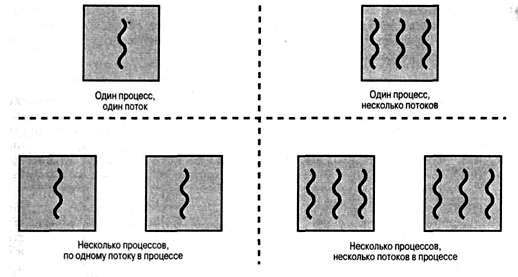
\includegraphics[width = 15cm]{1.jpg}
\end{center}
\noindent
\bf ВАЖНО: \rm Для понимания работы потоков необходимо помнить, что каждый поток имеет независимый от других потоков стек выполнения.

\begin{center}
  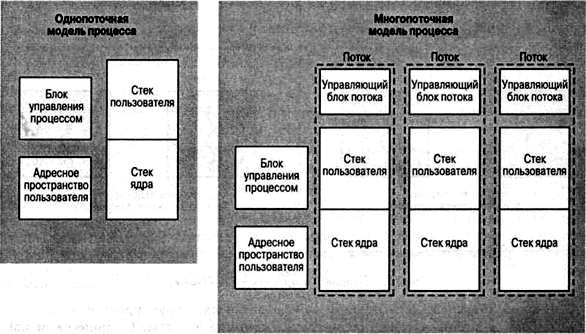
\includegraphics[width = 13cm]{2.jpg}
\end{center}
\noindent
В рамках процесса могут находиться один или несколько потоков, каждый из которых обладает следующими характеристиками:
\begin{enumerate}
  \item Состояние выполнения потока (выполняющийся, готовый к выполнению и т.д.);
  \item Сохраненный контекст не выполняющегося потока; один из способов рассмотрения потока — считать его независимым счетчиком команд, работающим в рамках процесса;
  \item Стек выполнения;
  \item Статическая память, выделяемая потоку для локальных переменных;
  \item Доступ к памяти и ресурсам процесса, которому этот поток принадлежит, этот доступ разделяется всеми потоками данного процесса.
\end{enumerate}
\vspace{1cm}
Потоки выполнения отличаются от традиционных процессов многозадачной операционной системы тем, что:
\begin{enumerate}
  \item Процессы, как правило, независимы, тогда как потоки выполнения существуют как составные элементы процессов;
  \item Процессы несут значительно больше информации о состоянии, тогда как несколько потоков выполнения внутри процесса совместно используют информацию о состоянии, а также память и другие вычислительные ресурсы;
  \item Процессы имеют отдельные адресные пространства, тогда как потоки выполнения совместно используют их адресное пространство;
  \item Процессы взаимодействуют только через предоставляемые системой механизмы связей между процессами;
  \item Переключение контекста между потоками выполнения в одном процессе, как правило, быстрее, чем переключение контекста между процессами.
\end{enumerate}
\subsection{\Large Системные вызовы для работы с потоками:}
\begin{center}
  \begin{tabular}{|p{4cm}|p{11cm}|}
  \hline
  pthread\_create & Создает новый поток \\
  \hline
  pthread\_self & Возвращает идентификатор текущего потока \\
  \hline
  pthread\_exit & Завершает поток \\
  \hline
  pthread\_kill & Посылает сигнал в поток \\
  \hline
  pthread\_join & Блокирует вызывающий поток до завершения потока \\
  \hline
  \end{tabular}
\end{center}

\subsubsection{\Large Системный вызов pthread\_create:}
\begin{verbatim}
include <pthread.h>
int pthread_create(pthread_t *tid, 
                   const pthread_attr_t *attr, 
                   void*(*func) (void*), 
                   void *arg);
\end{verbatim}
При успешном завершении идентификатор созданного потока помещается по адресу, указанному параметром tid. Атрибуты создаваемого потока передаются в attr. Если attr равен NULL, то используются параметры по умолчанию. Параметр func передает указатель на функцию следующего вида:
\begin{verbatim}
void thread_func(void*);
\end{verbatim}
Аргумент arg передается в функцию func.

\subsubsection{\Large Системный вызов pthread\_self:}
Возвращает идентификатор текущего потока.
\begin{verbatim}
#include <pthread.h>
pthread_t pthread_self();
\end{verbatim}

\subsubsection{\Large Системный вызов pthread\_exit.}
\begin{verbatim}
#include <pthread.h>
void pthread_exit(void *status);
\end{verbatim}
Функция pthread\_exit служит для завершения нити исполнения (thread'а) текущего процесса.\\\\
Функция никогда не возвращается в вызвавший ее thread. Объект, на который указывает параметр status, может быть впоследствии изучен в другой нити исполнения, например, в породившей завершившуюся нить. Поэтому он не должен указывать на динамический объект завершившегося thread'а.

\subsubsection{\Large Системный вызов pthread\_join:}
\begin{verbatim}
#include <pthread.h>
int pthread_join (pthread_t thread, void **status_addr);
\end{verbatim}
Описание функции:\\
Функция pthread\_join блокирует работу вызвавшей ее нити исполнения до завершения thread'а с идентификатором thread. После разблокирования в указатель, расположенный по адресу status\_addr, заносится адрес, который вернул завершившийся thread либо при выходе из ассоциированной с ним функции, либо при выполнении функции pthread\_exit(). Если нас не интересует, что вернула нам нить исполнения, в качестве этого параметра можно использовать значение NULL.\\\\
Возвращаемые значения:\\
\begin{tabular}{p{2cm}p{13cm}}
  \bf  0 & \rm при успешном завершении \\
  \bf >0 & \rm в случае ошибки \\
\end{tabular}
\\\\
В случае ошибки, возвращаемое значение определят код ошибки, описанный в файле errno.h. Значение системной переменной errno при этом не устанавливается.

\subsubsection{\Large Системный вызов pthread\_detach.}
\begin{verbatim}
#include <pthread.h>
int pthread_detach(pthread_t thread);
\end{verbatim}
Отсоединяет поток. По умолчанию все потоки создаются присоединенными. Это означает, что когда поток завершается его идентификатор и статус завершения сохраняются до тех пор, пока какой-либо поток данного процесса не вызовет pthread\_join. Если поток является отсоединенным, то после его завершения все ресурсы освобождаются.

\newpage
\section{\bf Лабораторная работа №4. FIFO}
Для организации потокового взаимодействия любых процессов в операционной системе UNIX применяется средство связи, получившее название FIFO (от First Input First Output) или именованный pipe. FIFO во всем подобен pipe, за одним исключением: доступ к FIFO процессы могут получать не через родственные связи, а через файловую систему. Для этого при создании FIFO на диске создается файл специального типа, обращаясь к которому процессы могут обмениваться информацией. Для создания FIFO используется системный вызов \sl mknod() \rm или существующая в некоторых версиях UNIX функция \sl mkfifo().\\\\
\rm \bf Важно! \rm При работе этих системных вызовов не происходит действительного выделения области адресного пространства операционной системы под именованный pipe, а только заводится файл-метка, существование которой позволяет осуществить реальную организацию FIFO в памяти при его открытии с помощью системного вызова \sl open().\\\\
После открытия FIFO ведет себя точно так же, как и pipe. Для дальнейшей работы с ним применяются системные вызовы \sl read(), write() и close(). \rm Время существования FIFO в адресном пространстве ядра операционной системы, как и в случае с pipe, не может превышать время жизни последнего из использовавших его процессов. Когда все процессы, работающие с FIFO, закрывают все файловые дескрипторы, ассоциированные с ним, система освобождает ресурсы, выделенные под FIFO. Вся непрочитанная информация теряется. В то же время файл-метка остается на диске и может использоваться для новой реальной организации FIFO в дальнейшем.\\\\
\bf Важно! \rm Системный вызов lseek() к FIFO не применим.

\subsection{\Large Использование системного вызова mknod() для создания FIFO.}
Прототип системного вызова:
\begin{verbatim}
#include <sys/stat.h>
#include <unistd.h>
int mknod(char *path, int mode, int dev);  
\end{verbatim}
Описание системного вызова:\\
Параметр \sl dev \rm является несущественным в нашей ситуации, и мы будем всегда задавать его равным 0.\\
Параметр \sl path \rm является указателем на строку, содержащую полное или относительное имя файла, который будет являться меткой FIFO на диске. Для успешного создания FIFO файла с таким именем перед вызовом существовать не должно.\\
Параметр \sl mode \rm устанавливает атрибуты прав доступа различных категорий пользователей к FIFO, аналогичные атрибутам задающим права доступа для файлов. Этот параметр задается как результат побитовой операции «или» значения S\_IFIFO и параметра mode.\\
При создании FIFO реально устанавливаемые права доступа получаются из стандартной комбинации параметра \sl mode \rm и маски создания файлов текущего процесса \sl umask, \rm именно – они равны \sl (0777 \& mode) \& ~umask.\\\\
\rm Возвращаемые значения:\\
При успешном создании FIFO системный вызов возвращает значение 0, при неуспешном – отрицательное значение.

\subsection{\Large Использование системного вызова mkfifo() для создания FIFO.}
Прототип функции:
\begin{verbatim}
#include <sys/stat.h>
#include <unistd.h>
int mkfifo(char *path, int mode);  
\end{verbatim}
Описание функции:\\
Функция mkfifo() предназначена для создания FIFO в операционной системе.\\
Параметр \sl path \rm является указателем на строку, содержащую полное или относительное имя файла, который будет являться меткой FIFO на диске. Для успешного создания FIFO файла с таким именем перед вызовом функции не должно существовать.\\
Параметр \sl mode \rm соответствует параметру mode системного вызова mknode().\\\\
Возвращаемые значения:\\
При успешном создании FIFO функция возвращаетзначение 0, при ошибке – отрицательное значение.\\
Важно понимать, что файл типа FIFO не служит для размещения на диске информации, которая записывается в FIFO. Эта информация располагается внутри адресного пространства операционной системы, а файл является только меткой.

\subsection{\Large Особенности поведения вызова open() при открытии FIFO.}
Системные вызовы read() и write() при работе с FIFO имеют те же особенности поведения, что и при работе с pipe. \\
Системный вызов open() при открытии FIFO также ведет себя несколько иначе, чем при открытии других типов файлов, что связано с возможностью блокирования выполняющих его процессов. \\
Если FIFO открывается только для чтения, и флаг O\_NDELAY не задан, то процесс, осуществивший системный вызов, блокируется до тех пор, пока какой-либо другой процесс не откроет FIFO на запись. \\
Если флаг O\_NDELAY задан, то возвращается значение файлового дескриптора, ассоциированного с FIFO. \\
Если FIFO открывается только для записи, и флаг O\_NDELAY не задан, то процесс, осуществивший системный вызов, блокируется до тех пор, пока какой-либо другой процесс не откроет FIFO на чтение.\\
Если флаг O\_NDELAY задан, то констатируется возникновение ошибки и возвращается значение -1. \\
Задание флага O\_NDELAY в параметрах системного вызова open() приводит и к тому, что процессу, открывшему FIFO, запрещается блокировка при выполнении последующих операций чтения из этого потока данных и записи в него. \\\\
Если процесс записывает данные в FIFO, с которым не взаимодействует в режиме чтения ни один другой процесс, то ядро посылает в него сигнал SIGPIPE, для уведомления. Если процесс пытается прочитать данные из FIFO, с которым ни один процесс не взаимодействует в режиме записи, то он прочитает оставшиеся (если они там были) данные и признак конца файла. \\
Таким образом, если два процесса взаимодействуют через FIFO записывающий процесс после завершения работы должен закрыть свой дескриптор FIFO для того, чтобы читающий процесс получил признак конца файла.

\newpage
\section{\bf Лабораторная работа №5. Разделяемая память}
Разделяемую память \sl (англ. Shared memory) \rm применяют для того, чтобы увеличить скорость прохождения данных между процессами. В обычной ситуации обмен информацией между процессами проходит через ядро. Техника разделяемой памяти позволяет осуществить обмен информацией не через ядро, а используя некоторую часть виртуального адресного пространства, куда помещаются и откуда считываются данные. После создания разделяемого сегмента памяти любой из пользовательских процессов может подсоединить его к своему собственному виртуальному пространству и работать с ним, как с обычным сегментом памяти. Недостатком такого обмена информацией является отсутствие каких бы то ни было средств синхронизации, однако для преодоления этого недостатка можно использовать технику семафоров.\\\\
Для работы с разделяемой памятью используются системные вызовы:
\begin{itemize}
  \item shmget — создание сегмента разделяемой памяти;
  \item shmctl — установка параметров;
  \item shmat — подсоединение сегмента памяти
  \item shmdt — отсоединение сегмента.
\end{itemize}

\subsection{\Large Получение IPC идентификатора.}
\begin{verbatim}
#include <sys/ipc.h>
key_t ftok(const char *path, int id);
\end{verbatim}
ftok использует файл с именем pathname (которое должно указывать на существующий файл к которому есть доступ) и младшие 8 бит id (который должен быть отличен от нуля) для создания ключа с типом key\_t.\\\\
Возвращаемое значение одинаково для всех имен, указывающих на один и тот же файл при одинаковом значении id. Возвращаемое значение должно отличаться, когда (одновременно существующие) файлы или идентификаторы проекта различаются.

\subsection{\Large Системный вызвод shmget.}
\begin{verbatim}
#include <sys/ipc.h>
#include <sys/shm.h>
int shmget(key_t key, int size, int shmflg);
\end{verbatim}
\sl shmget() \rm возвращает идентификатор разделяемому сегменту памяти, соответствующий значению аргумента \sl key.\\
\rm Создается новый разделяемый сегмент памяти с размером \sl size \rm округленным до размера, кратного PAGE\_SIZE), если значение key равно IPC\_PRIVATE или если значение \sl key \rm не равно IPC\_PRIVATE и нет идентификатора, соответствующего key; причем, выражение shmflg \& IPC\_CREAT истинно.\\
Поле \sl shmflg \rm состоит из:\\\\
\begin{tabular}{|p{3cm}|p{12cm}|}
  \hline
  IPC\_CREAT & служит для создания нового сегмента. Если этого флага нет, то функция \sl shmget() \rm будет искать сегмент, соответствующий ключу \sl key \rm и затем проверит, имеет ли пользователь права на доступ к сегменту. \\
  \hline
  IPC\_EXCL & используется совместно с IPC\_CREAT для того, чтобы не создавать существующий сегмент заново.\\
  \hline
\end{tabular}\\
Если создается новый сегмент, то права доступа копируются из shmflg в \sl shm\_perm, \rm являющийся членом структуры \sl shmid\_ds, \rm которая определяет сегмент. \\\\
Структура \sl shmid\_ds \rm имеет такую форму:
\begin{verbatim}
struct shmid_ds 
{
  struct ipc_perm shm_perm; /* права операции */
  int shm_segsz; /* размер сегмента (в байтах) */
  time_t shm_atime; /* время последнего подключения */
  time_t shm_dtime; /* время последнего отключения */
  time_t shm_ctime; /* время последнего изменения */
  unsigned short shm_cpid; /* идентификатор процесса создателя */
  unsigned short shm_lpid; /* идентификатор последнего 
                                            пользователя */
  short shm_nattch; /* количество подключений */
};

struct ipc_perm 
{
  key_t key;
  ushort uid; /* действующие идентификаторы владельца и 
                                    группы euid и egid */
  ushort gid;
  ushort cuid; /* действующие идентификаторы 
                              создателя euid и egid */
  ushort cgid;
  ushort mode; /* младшие 9 битов shmflg */
  ushort seq; /* номер последовательности */
};
\end{verbatim}
При ошибке переменная \sl errno \rm приобретает одно из следующих значений:
\begin{tabular}{p{3cm}p{12cm}}
EINVAL & если создается новый сегмент, а size < SHMMIN или size > SHMMAX, либо новый сегмент не был создан. Сегмент с данным ключем существует, но size больше чем размер этого сегмента.\\\\
EEXIST & если значение IPC\_CREAT | IPC\_EXCL было указано, а сегмент уже существует.\\\\
ENOSPC & если все возможные идентификаторы сегментов уже распределены (SHMMNI) или если размер выделяемого сегмента превысит системные лимиты (SHMALL).\\\\
ENOENT & если не существует сегмента для ключа key, а значение IPC\_CREAT не указано.\\\\
EACCES & если у пользователя нет прав доступа к сегменту разделяемой памяти.\\\\
ENOMEM & если в памяти нет свободного для сегмента пространства.\\\\
\end{tabular}

\subsection{\Large Системный вызов shmat.}
\begin{verbatim}
#include <sys/types.h>
#include <sys/shm.h>
void *shmat(int shmid, const void *shmaddr, int shmflg);
\end{verbatim}
Функция shmat подстыковывает сегмент разделяемой памяти \sl shmid \rm к адресному пространству вызывающего процесса. Адрес подстыковываемого сегмента определяется \sl shmaddr \rm с помощью одного из перечисленных ниже критериев:
\begin{itemize}
  \item Если \sl shmaddr \rm равен \bf NULL, \rm то система выбирает для подстыкованного сегмента подходящий (неиспользованный) адрес.
  \item Если \sl shmaddr \rm не равен \bf NULL, \rm а в поле \sl shmflg \rm включен флаг SHM\_RND, то подстыковка производится по адресу \sl shmaddr, \rm округленному вниз до ближайшего кратного SHMLBA. В противном случае \sl shmaddr \rm должен быть округленным до размера страницы адресом, к которому производится подстыковка.
  \item Если в поле \sl shmflg включен флаг SHM\_RDONLY, то подстыковываемый сегмент будет доступен только для чтения, и вызывающий процесс должен иметь права на чтение этого сегмента. Иначе, сегмент будет доступен для чтения и записи, и у процесса должны быть соответствующие права. Сегментов "только-запись" не существует.
  \item Флаг SHM\_REMAP (специфичный для Linux) может быть указан в \sl shmflg \rm для обозначения того, что распределение сегмента должно замещать любые существующие распределения в диапазоне, начиная с \sl shmaddr \rm и до размера сегмена. (Обычно выдается ошибка EINVAL если уже существует распределение в этом диапазоне адресов.) В этом случае \sl shmaddr \rm не должно быть равно \bf NULL.
  \item \rm Значение \sl brk \rm вызывающего процесса подстыковкой не изменяется. При завершении работы процесса сегмент будет отстыкован. Один и тот же сегмент может быть подстыкован в адресное пространство процесса несколько раз, как "только для чтения", так и в режиме "чтение-запись".
\end{itemize}
При удачном выполнении системный вызов shmat обновляет содержимое структуры shmid\_ds, связанной с разделяемым сегментом памяти, следующим образом:
\begin{itemize}
  \item shm\_atime устанавливается в текущее время;
  \item shm\_lpid устанавливается в идентификатор вызывающего процесса;
  \item shm\_nattch увеличивается на 1.
\end{itemize}
Заметьте, что пристыковка производится и в том случае, если пристыковываемый сегмент помечен на удаление.

\subsection{\Large Системный вызов shmdt.}
\begin{verbatim}
int shmdt(const void *shmaddr);
\end{verbatim}
Функция shmdt отстыковывает сегмент разделяемой памяти, находящийся по адресу \sl shmaddr, \rm от адресного пространства вызвающего процесса. Отстыковываемый сегмент должен быть среди пристыкованных ранее функцией shmat. Параметр \sl shmaddr \rm должен быть равен значению, которое возвратила соответствующая функция shmat.\\\\
При удачном выполнении системный вызов shmdt обновляет содержимое структуры shmid\_ds, связанной с разделяемым сегментом памяти, следующим образом:
\begin{itemize}
  \item shm\_dtime устанавливается в текущее время;
  \item shm\_lpid устанавливается в идентификатор вызывающего процесса;
  \item shm\_nattch уменьшается на 1. Если это значение становится равным 0, а сегмент помечен на удаление, то сугмент удаляется из памяти. Эта функция освобождает занятую ранее этим сегментом область памяти в адресном пространстве процесса.
\end{itemize}

\subsection{\Large Системный вызов shtctl.}
\begin{verbatim}
#include <sys/ipc.h>
#include <sys/shm.h>
int shmctl(int shmid, int cmd, struct shmid_ds *buf);
\end{verbatim}
\sl shmctl() \rm позволяет пользователю получать информацию о разделяемых сегментах памяти, устанавливать владельца, группу разделяемого сегмента, права на него; эта функция может также удалить сегмент. Информация о сегменте, которая находится в \sl shmid, \rm возвращается в структуру shmid\_ds:
\begin{verbatim}
struct shmid_ds 
{
  struct ipc_perm shm_perm; /* права на выполнение операции */
  int shm_segsz; /* размер сегмента (в байтах) */
  time_t shm_atime; /* время последнего подключения */
  time_t shm_dtime; /* время последнего отключения */
  time_t shm_ctime; /* время последнего изменения структуры */
  unsigned short shm_cpid; /* идентификатор процесса создателя */
  unsigned short shm_lpid; /* идентификатор процесса, 
                              подключавшегося последним */
  short shm_nattch; /* количество текущих подключений сегмента */
  ...
};
\end{verbatim}
Выделенные поля в \sl shm\_perm \rm могут быть установлены следующим образом:
\begin{verbatim}
struct ipc_perm {
  key_t key;
  ushort uid; /* owner euid and egid */
  ushort gid;
  ushort cuid; /* creator euid and egid */
  ushort cgid;
  ushort mode; /* lower 9 bits of access modes */
  ushort seq; /* sequence number */
};
\end{verbatim}
\vspace{0.5cm}
Значения аргумента \sl cmds \rm могут быть следующими:\\\\
\begin{tabular}{|p{3cm}|p{12cm}|}
  \hline
  \bf IPC\_STAT & \rm используется для копирования информации о сегменте в буфер \sl buf. \rm Пользователь должен иметь права на чтение сегмента \bf read.\rm \\
  \hline
  \bf IPC\_SET & \rm используется для применения пользовательских изменений к содержимому полей \sl uid, gid \rm или \sl mode в структуре \sl shm\_perms. \rm Используются только младшие 9 битов \sl mode. \rm Поле \sl shm\_ctime тоже обновляется. Пользователь должен быть владельцем, создателем или суперпользователем процесса. \\
  \hline
  \bf IPC\_RMID & \rm используется для пометки сегмента как удаленного. Сегмент будет удален после отключения (например, когда поле \sl shm\_nattch \rm ассоциированной структуры \sl shmid\_ds \rm равно нулю). Пользователь должен быть владельцем, создателем или суперпользователем процесса.\\
  \hline
\end{tabular}
\vspace{0.5cm}

Пользователь \bf должен \rm удостовериться, что сегмент удален; иначе страницы, которые не были удалены, останутся в памяти или в разделе подкачки. Также процессы с соответствующими привилегиями могут предотвратить или разрешить подкачку разделяемого сегмента памяти при помощи следующих команд cmds (применимо только для Linux):\\\\
\begin{tabular}{|p{5cm}|p{10cm}|}
  \hline
  \bf SHM\_LOCK & \rm запретить подкачку разделяемого сегмента памяти. После блокировки страницы должны находиться в памяти.\\
  \hline
  \bf SHM\_UNLOCK & \rm разрешить подкачку сегмента.\\
  \hline
\end{tabular}
\vspace{0.5cm}

Процессы, которым разрешено использовать\\\bf SHM\_LOCK \rm и \bf SHM\_UNLOCK \\\rm при запуске их с возможностью \\\bf CAP\_IPC\_LOCK \rm (обычно выдаваемой только для \bf root) \rm или если их текущий лимит ресурсов \\\bf RLIMIT\_MEMLOCK \rm не равен нулю.

\newpage
\section{\bf Лабораторная работа №6. Взаимные исключения}
При наличии нескольких потоков управления, совместно использующих одни и те же данные, необходимо гарантировать, что каждый из потоков будет видеть эти данные в непротиворечивом состоянии. Если каждый из потоков использует переменные, которые не используются в других потоках, то проблем не возникает. Аналогично, если переменная доступна одновременно нескольким потокам только для чтения, то здесь так же отсутствует проблема сохранения непротиворечивости. Однако, если один поток изменяет значение переменной, читать или изменять которое могут также другие потоки, то необходимо синхронизировать доступ к переменной, чтобы гарантировать, что потоки не будут получать неверное значение переменной при одновременном доступе к ней.\\\\
Когда поток изменяет значение переменной, существует потенциальная опасность, что другой поток может прочитать еще не до конца записанное значение. На аппаратных платформах, где запись в память осуществляется более чем за один цикл, может произойти так, что между двумя циклами записи вклинится цикл чтения. Разумеется, такое поведение во многом зависит от аппаратной архитектуры, но при написании переносимых программ мы не можем полагаться на то, что они будут выполняться только на определенной платформе.\\\\
Мы можем защитить данные и ограничить доступ к ним одним потоком в один момент времени с помощью интерфейса взаимоисключений (mutual exclusion) pthreads. Мьютекс (mutex) – это фактически блокировка, которая устанавливается (запирается) перед обращением к разделяемому ресурсу и снимается (отпирается) после выполнения требуемой последовательности операций. Если мьютекс заперт, то любой другой поток, который попытается запереть его, будет заблокирован до тех пор, пока мьютекс не будет отперт.\\\\
Если в момент, когда отпирается мьютекс, заблокированными окажутся несколько потоков, все они будут запущены и первый из них, который успеет запереть мьютекс, продолжит работу. Все остальные потоки обнаружат, что мьютекс по-прежнему заперт, и опять перейдут в режим ожидания. Таким образом, доступ к ресурсу сможет получить одновременно только один поток.\\\\
Такой механизм взаимоисключений будет корректно работать только при условии, что все потоки приложения будут соблюдать одни и те же правила доступа к данным. Операционная система никак не упорядочивает доступ к данным. Если мы позволим одному потоку производить действия с разделяемыми данными, предварительно не ограничив доступ к ним, то остальные потоки могут обнаружить эти данные в противоречивом состоянии, даже если перед обращением к ним будут устанавливать блокировку.\\\\
Переменные-мьютексы определяются с типом pthread\_mutex\_t. Прежде чем использовать переменную мьютекс, мы должны сначала инициализировать ее, записав в нее значение константы PTHREAD\_MUTEX\_INITIALIZER (только для статически размещаемых мьютексов) или вызвав функцию pthread\_mutex\_init.\\\\
Системные вызовы работы с mutex:
\begin{itemize}
  \item pthread\_mutex\_init
  \item pthread\_mutex\_destroy
  \item pthread\_mutex\_lock
  \item pthread\_mutex\_trylock
  \item pthread\_mutex\_unlock
\end{itemize}

\subsection{\Large Системный вызов pthread\_mutex\_init.}
\begin{verbatim}
#include <pthread.h>
int pthread_mutex_init(pthread_mutex_t *restrict mutex, 
                       const pthread_mutexattr_t *restrict attr);
\end{verbatim}
Инциализирует мьютекс переданный параметром mutex. Для того, чтобы использовать параметры по умолчанию необходимо вместо attr передать NULL.

\subsection{\Large Системный вызов pthread\_mutex\_destroy.}
\begin{verbatim}
#include <pthread.h>
int pthread_mutex_destroy(pthread_mutex_t *restrict mutex);
\end{verbatim}
Уничтожает мьютекс.

\subsection{\Large Системный вызов pthread\_mutex\_lock.}
\begin{verbatim}
#include <pthread.h>
int pthread_mutex_lock(pthread_mutex_t *mutex);
\end{verbatim}
Блокирует мьютекс. Если мьютекс уже заблокирован, то вызывающий поток блокируется.

\subsection{\Large Системный вызов pthread\_mutex\_trylock.}
\begin{verbatim}
#include <pthread.h>
int pthread_mutex_trylock(pthread_mutex_t *mutex);
\end{verbatim}
Если к моменту вызова этой функции мьютекс будет отперт, функция запрет мьютекс и вернет значение 0. В противном случае pthread\_mutex\_trylock вернет код ошибки EBUSY. Вызывающий поток при в этом случае не плокируется.

\subsection{\Large Системный вызов pthread\_mutex\_unlock.}
\begin{verbatim}
#include <pthread.h>
int pthread_mutex_unlock(pthread_mutex_t *mutex);
\end{verbatim}
Разблокирует мьютекс.

\newpage
\section{\bf Лабораторная работа №7. Условные переменные}
Условные переменные используются для того, чтобы заблокировать потоки до выполнения определенных условий. Условные переменные применяются в сочетании с мьютексам, чтобы несколько потоков могли ожидать момента выполнения одного условия. Это можно сделать несколькими способами. Сначала поток блокирует мьютекс, но и сам блокируется до момента выполнения условия. На то время, пока поток заблокирован, установленная им блокировка мьютекса автоматически снимается. Когда другой поток выполняет поставленное условие, он дает условной переменной сигнал (не имеющий отношения к сигналам unix) о разблокировании первого потока. После блокировки потока мьютекс автоматически устанавливается и первый поток повторно проверяет условие. Если оно не выполняется, поток опять блокируется переменной. Если условие выполняется, поток разблокирует мьютекс и выполняется дальше.\\\\
Системные вызовы для работы с условными переменными:
\begin{itemize}
  \item pthread\_cond\_init
  \item pthread\_cond\_wait
  \item pthread\_cond\_timedwait
  \item pthread\_cond\_signal
  \item pthread\_cond\_broadcast
  \item pthread\_cond\_destroy
\end{itemize}

\subsection{\Large Системный вызов pthread\_cond\_init.}
\begin{verbatim}
#include <pthread.h>
int pthread_cond_init (pthread_cond_t *cond,
                       const pthread_condattr_t *attr);

pthread_cond_t cond = PTHREAD_COND_INITIALIZER;
\end{verbatim}
Инициализирует атрибутный объект условной переменной, заданный параметром attr, значениями, действующими по умолчанию для всех атрибутов, определенных реализацией.

\subsection{\Large Системный вызов pthread\_cond\_wait.}
\begin{verbatim}
#include <pthread.h>
int pthread_cond_wait(pthread_cond_t *restrict cond, 
                      pthread_mutex_t *restrict mutex);
\end{verbatim}
При вызове pthread\_cond\_wait мьютекс должен быть захвачен, в противном случае результат не определен. Pthread\_cont\_wait освобождает мьютекс и блокирует нить до момента вызова другой нитью pthread\_cond\_signal. После пробуждения wait пытается захватить мьютекс; если это не получается, он блокируется до того момента, пока мьютекс не освободят.

\subsection{\Large Системный вызов pthread\_cond\_timedwait}
\begin{verbatim}
#include <pthread.h>
int pthread_cond_timedwait(pthread_cond_t *restrict cond,  
                           pthread_mutex_t *restrict mutex,
                           const struct timespec *restrict abstime);
\end{verbatim}
Аналогично pthread\_cond\_wait, но задается время ожидания разблокировки.

\subsection{\Large Системный вызов pthread\_cond\_signal.}
\begin{verbatim}
#include <pthread.h>
int pthread_cond_signal(pthread_cond_t *cond);
\end{verbatim}
Разблокирует поток, заблокированный вызовом pthread\_cond\_wait().

\subsection{\Large Системный вызов pthread\_cond\_broadcast.}
\begin{verbatim}
#include <pthread.h>
int pthread_cond_broadcast(pthread_cond_t *cond);
\end{verbatim}
Разблокирует \underline{все} потоки, заблокированные вызовом pthread\_cond\_wait().\\

\subsection{\Large Системный вызов pthread\_cond\_destroy.}
\begin{verbatim}
int pthread_cond_destroy(pthread_cond_t *cond);
\end{verbatim}
Уничтожает условную переменную.

\newpage
\section{\bf Лабораторная работа №8. Блокировки чтения-записи}
Блокировки чтения-записи похожи на мьютексы, за исключением того, что они допускают более высокую степень параллелизма. Мьютексы могут иметь всего два состояния, закрытое и открытое, и только один поток может владеть мьютексом в каждый момент времени. Блокировки чтения-записи могут иметь три состояния: \sl режим блокировки для чтения, режим блокировки для записи и отсутствие блокировки. \rm Режим блокировки для записи может установить только один поток, но установка режима блокировки для чтения доступна нескольким потокам одновременно.\\\\
Если блокировка чтения-записи установлена в режиме блокировки для записи, все потоки, которые будут пытаться захватить эту блокировку, будут приостановлены до тех пор, пока блокировка не будет снята. Если блокировка чтения-записи установлена в режиме блокировки для чтения, все потоки, которые будут пытаться захватить эту блокировку для чтения, получат доступ к ресурсу, но если какой-либо поток попытается установить режим блокировки для записи, он будет приостановлен до тех пор, пока не будет снята последняя блокировка для чтения. Различные реализации блокировок чтения-записи могут значительно различаться, но обычно, если блокировка для чтения уже установлена и имеется поток, который пытается установить блокировку для записи, то остальные потоки, которые пытаются получить блокировку для чтения, будут приостановлены. Это предотвращает возможность блокирования пишущих потоков непрекращающимися запросами на получение блокировки для чтения.\\\\
Блокировки чтения-записи прекрасно подходят для ситуаций, когда чтение данных производится намного чаще, чем запись. Когда блокировка чтения-записи установлена в режиме для записи, можно безопасно выполнять модификацию защищаемых ею данных, поскольку только один поток может владеть блокировкой для записи. Когда блокировка чтения-записи установлена в режиме для чтения, защищаемые ею данные могут быть безопасно прочитаны несколькими потоками, если эти потоки смогли получить блокировку для чтения.\\\\
Блокировки чтения-записи еще называют совместноисключающими блокировками. Когда блокировка чтения-записи установлена в режиме для чтения, то говорят, что блокировка находится в режиме совместного использования. \\\\
Когда блокировка чтения-записи установлена в режиме для записи, то говорят, что блокировка находится в режиме исключительного использования.\\

\subsection{\Large Системный вызов pthread\_rwlock\_init.}
\begin{verbatim}
#include <pthread.h>
int pthread_rwlock_init(pthread_rwlock_t *restrict rwlock, 
                        const pthread_rwlockattr_t *restrict attr);
                        
pthread_rwlock_t rwlock = PTHREAD_RWLOCK_INITIALIZER;
\end{verbatim}
Функция pthread\_rwlock\_init инициализирует блокировку чтения-записи. Если в аргументе attr передается пустой указатель, блокировка инициализируется с атрибутами по умолчанию.

\subsection{\Large Системный вызов pthread\_rwlock\_destroy.}
\begin{verbatim}
#include <pthread.h>
int pthread_rwlock_destroy(pthread_rwlock_t *rwlock);
\end{verbatim}
Перед освобождением памяти, занимаемой блокировкой чтения-записи, нужно вызвать функцию pthread\_rwlock\_destroy, чтобы освободить все занимаемые блокировкой ресурсы.

\subsection{\Large Системный вызов pthread\_rwlock\_rdlock.}
\begin{verbatim}
#include <pthread.h>
int pthread_rwlock_rdlock(pthread_rwlock_t *rwlock);
\end{verbatim}
Заблокировать ресурс для чтения.

\subsection{\Large Системный вызов pthread\_rwlock\_wrlock.}
\begin{verbatim}
#include <pthread.h>
int pthread_rwlock_wrlock(pthread_rwlock_t *rwlock);
\end{verbatim}
Заблокировать ресурс для записи.

\subsection{\Large Системный вызов pthread\_unlock\_wrlock.}
\begin{verbatim}
#include <pthread.h>
int pthread_rwlock_unlock(pthread_rwlock_t *rwlock);
\end{verbatim}
Снять блокировку чтения-записи.

\subsection{\Large Системный вызов pthread\_tryrdlock\_wrlock.}
\begin{verbatim}
#include <pthread.h>
int pthread_rwlock_tryrdlock(pthread_rwlock_t *rwlock);
\end{verbatim}
Попытаться заблокировать ресурс для чтения.

\subsection{\Large Системный вызов pthread\_trywrlock\_wrlock.}
\begin{verbatim}
#include <pthread.h>
int pthread_rwlock_trywrlock(pthread_rwlock_t *rwlock);
\end{verbatim}
Попытаться заблокировать ресурс для записи.

\newpage
\section{\bf Список литературы.}
\begin{enumerate}
  \item Стивенс, У. UNIX: взаимодествие процессов. СПб. : Питер, 2003. стр. 576.
  \item Теренс, Чан. Системной программирование на C++ для UNIX. К. : Издательская группа BHV, 1997. стр. 592. ISNB 5-7315-0013-4.
  \item Стивенс, У. UNIX: разработка сетевых приложений. СПб. : Питер, 2003. стр. 1088.
  \item Свободная энциклопедия "Википедия". [В Интернете]
\end{enumerate}

\end{document}
